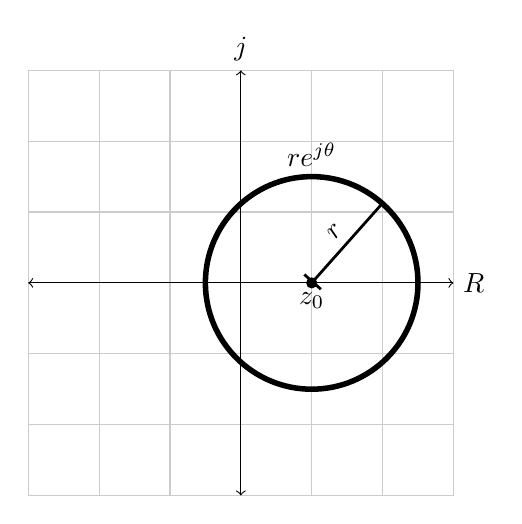
\begin{tikzpicture} [scale=0.9]
    \draw[thin,gray!40] (-3,-3) grid (3,3);
    \draw[<->] (-3,0)--(3,0) node[right] {$R$};
    \draw[<->] (0,-3)--(0,3) node[above]{$j$};
    \draw[line width=2pt] (1,0) circle(1.5);
    \draw[] (1,1.5) node[above]{$re^{j\theta}$};
    \draw[fill=black] (1,0) circle(2pt) node[below]{$z_0$};
    \draw[line width=1pt,black,|-|] (1,0)--(2,1.125) node[midway,above,sloped]{$r$};
\end{tikzpicture}
\caption{Circunferencia en el plano complejo de centro $z_0$}